%%%%%%%%%%%%%%%%%%%%%%%%%%%%%%%%%%%%%%%%%%%%%%%%%%%%%%%%%%%%%%%%%%%%%
% LaTeX Template: Project Titlepage Modified (v 0.1) by rcx
%
% Original Source: http://www.howtotex.com
% Date: February 2014
% 
% This is a title page template which be used for articles & reports.
% 
% This is the modified version of the original Latex template from
% aforementioned website.
% https://www.overleaf.com/12873736hqjppcbqmmgw#/49189815/
%%%%%%%%%%%%%%%%%%%%%%%%%%%%%%%%%%%%%%%%%%%%%%%%%%%%%%%%%%%%%%%%%%%%%%

\documentclass[12pt]{report}
\usepackage[a4paper]{geometry}
\usepackage[myheadings]{fullpage}
\usepackage{fancyhdr}
\usepackage{lastpage}
\usepackage{graphicx, wrapfig, subcaption, setspace, booktabs}
\usepackage[T1]{fontenc}
\usepackage[font=small, labelfont=bf]{caption}
\usepackage{fourier}
\usepackage[protrusion=true, expansion=true]{microtype}
\usepackage[english]{babel}
\usepackage{sectsty}
\usepackage{url, lipsum}
\usepackage{tikz}
\usetikzlibrary{arrows,calc,positioning}

\tikzstyle{na}=[draw,minimum size=6em,text centered,text width=3.cm]
\tikzstyle{nb}=[draw,text centered,text width=3.cm,minimum width=4cm,minimum height=4cm,minimum size=6em]



\newcommand{\HRule}[1]{\rule{\linewidth}{#1}}
\onehalfspacing
\setcounter{tocdepth}{5}
\setcounter{secnumdepth}{5}

%-------------------------------------------------------------------------------
% HEADER & FOOTER
%-------------------------------------------------------------------------------
\pagestyle{fancy}
\fancyhf{}
\setlength\headheight{15pt}
\fancyhead[L]{University of Alberta}
\fancyfoot[R]{Page \thepage\ of \pageref{LastPage}}
%-------------------------------------------------------------------------------
% TITLE PAGE
%-------------------------------------------------------------------------------

\begin{document}

\title{ \normalsize \textsc{CMPUT 501 project}
		\\ [2.0cm]
		\HRule{0.5pt} \\
		\LARGE \textbf{\uppercase{Realtime Hand Gesture Recognition using Principal Component analysis based on skin colour segmentation}}
		\HRule{2pt} \\ [0.5cm]
		\normalsize \today \vspace*{5\baselineskip}}

\date{}

\author{
		Elizaveta Kharlova \\
		Student ID: 1403693 \\
        Nazmus Sakib\\
        Student ID: 1546701}

\maketitle
\tableofcontents
\newpage

%-------------------------------------------------------------------------------
% Section title formatting
\sectionfont{\scshape}
%-------------------------------------------------------------------------------

%-------------------------------------------------------------------------------
% BODY
%-------------------------------------------------------------------------------

\section*{Introduction}
Gesture recognition is one of the current problems in HCI (Human Computer Interface). Principal Component Analysis (PCA) is a computationally friendly and robust way to perform image recognition. This method has been used to perform face recognition in [3]. This can be applied to gesture recognition in real time. The main challenges of this approach are reducing of variance between the images in order to improve recognition, decreasing computational complexity, and selecting the training set. 

\addcontentsline{toc}{section}{Introduction}
\section*{Procedure}
\addcontentsline{toc}{section}{Procedure}
The process consisted of two main parts: training and recognition. In the training part, images were processed with segmentation and PCA in order to form a basis set. In the recognition part, each new frame was processed and projected onto the basis in order to produce a guess. This procedure is similar to [1].\\
\newline
Nazmus Sakib was responsible for the segmentation. Elizaveta Kharlova was responsible for the PCA.

\subsection*{Segmentation}
Segmentation is a very important part before the recognition. The accuracy of the PCA recognizer largely depends on proper segmentation. In our system we tried to get the grayscale image of hand subtracting the background.\\
The input video was captured in RGB. Then it was downsized with nearest neighbor interpolation. We chose nearest neighbor because it is fast despite the reduction of quality of the image. Each of the RGB components were scaled like the grayscale in order to compensate the illumination. This uniform scaling helps thresholding the skin color and subtracting the background. The thresholding was done on YCbCr image to form a new binary image. The binary images can show head, hands and any regions that look same as skin color.Then we use a binary label set algorithm to get regions.So the regions of interest were bounded with bounding box procedures and sorted with respect to area Figure (\ref{fig:Binaryimg}). In our system we take the box with the largest area where we assume that the human hand will be closer to the camera than his head.\\
\begin{figure}
\centering
\begin{subfigure}{.18\textwidth}
  \centering
  \includegraphics[width=1\linewidth]{all_5.jpg}
  \label{fig:sb1}
\end{subfigure}%
\begin{subfigure}{.18\textwidth}
  \centering
  \includegraphics[width=1\linewidth]{all_4.jpg}
  \label{fig:sb2}
\end{subfigure}
\begin{subfigure}{.18\textwidth}
  \centering
  \includegraphics[width=1\linewidth]{all_3.jpg}
  \label{fig:sb3}
\end{subfigure}
\begin{subfigure}{.18\textwidth}
  \centering
  \includegraphics[width=1\linewidth]{all_2.jpg}
  \label{fig:sb4}
\end{subfigure}
\begin{subfigure}{.18\textwidth}
  \centering
  \includegraphics[width=1\linewidth]{all_1.jpg}
\end{subfigure}
\\
\begin{subfigure}{.18\textwidth}
  \centering
  \includegraphics[width=1\linewidth]{hand_5.jpg}
  \caption{"5"}
  \label{fig:s1}
\end{subfigure}%
\begin{subfigure}{.18\textwidth}
  \centering
  \includegraphics[width=1\linewidth]{hand_4.jpg}
  \caption{"4"}
  \label{fig:s2}
\end{subfigure}
\begin{subfigure}{.18\textwidth}
  \centering
  \includegraphics[width=1\linewidth]{hand_3.jpg}
  \caption{"3"}
  \label{fig:s3}
\end{subfigure}
\begin{subfigure}{.18\textwidth}
  \centering
  \includegraphics[width=1\linewidth]{hand_2.jpg}
  \caption{"2"}
  \label{fig:s4}
\end{subfigure}
\begin{subfigure}{.18\textwidth}
  \centering
  \includegraphics[width=1\linewidth]{hand_1.jpg}
  \caption{"1"}
  \label{fig:s5}
\end{subfigure}
\caption{Hand Image Segmentation}
\label{fig:Binaryimg}
\end{figure}
Next we cropped the image based on the boundary. Since the content in the box depends on skin color thresholding, there are some gaps in between the regions. So we used flood filling algorithm to fill the holes inside the hand image. Now we took the grayscale pixel corresponding to the binary image. This process is a repetitive over each frame of the video sequence. The images were passed into PCA process for recognition. The following Figure(\ref{fig:segmentation}) shows the activity diagram of the whole procedure.
\begin{figure}[!htb]
    
    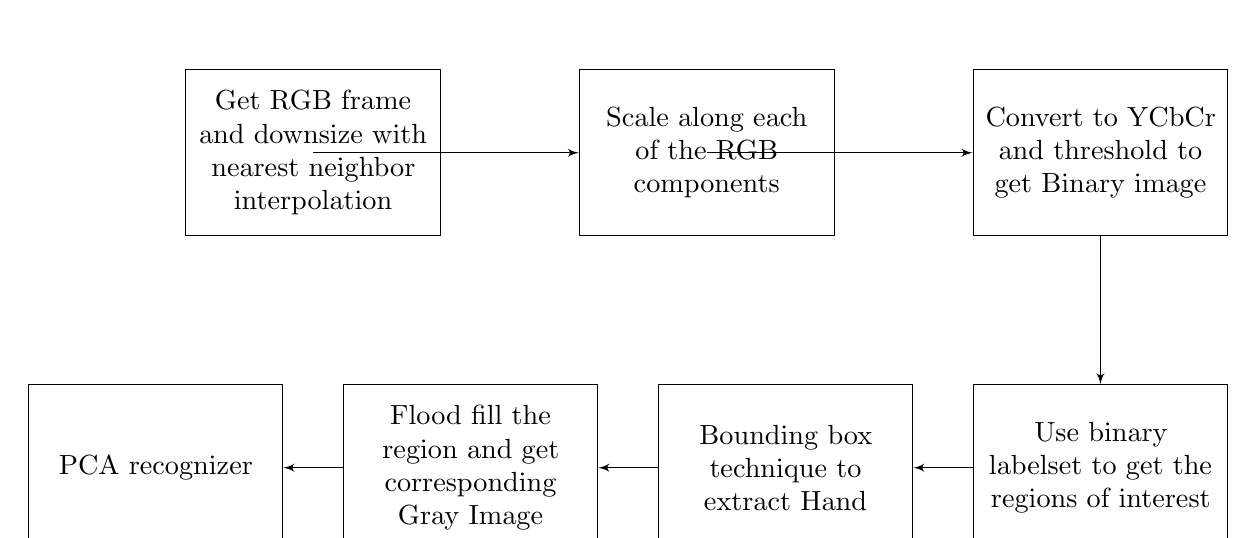
\begin{tikzpicture}[
      >=latex',
      auto
    ]
   
     \node [nb] (n1) [node distance=0cm] {Get RGB frame and downsize with nearest neighbor interpolation};
     \node [na] (n2) [node distance=5cm,right of=n1] {Scale along each of the RGB components };
	 \node [na] (n3) [node distance=5cm,right of=n2] {Convert to YCbCr and threshold to get Binary image};
     \node [na] (n4) [node distance=4cm,below of=n3] {Use binary labelset to get the regions of interest};
	 \node [na] (n5) [node distance=4cm,left of=n4] {Bounding box technique to extract Hand};
     \node [na] (n6) [node distance=4cm,left of=n5] {Flood fill the region and get corresponding Gray Image};
     \node [na] (n7) [node distance=4cm,left of=n6] {PCA recognizer};

      \draw[->] (n1) |- (n2);
      \draw[->] (n2) |- (n3);
      \draw[->] (n3) -- (n4);
      \draw[->] (n4) -- (n5);
      \draw[->] (n5) -- (n6);
      \draw[->] (n6) -- (n7);
    \end{tikzpicture}
    \caption{Segmentation Activity Digram}
    \label{fig:segmentation}
  \end{figure}


\subsection*{PCA}
Once the segmented grayscale images were loaded into one matrix, they were resized to an arbitrary average size (nxm) of the received images (here 100x80). They then were passed onto the PCA processing. This procedure is similar to the one described in [2] and [3].\\
% Include reference to the PCA papers. 
The first step was to rearrange each image such that it forms a column in the following way, where k is the number of images
\begin{equation}\label{rearrange_matrix}
    N_{nxmxk} = [Y^1_{nxm} Y^2_{nxm} ...] => M_{(nxm)xk} = [I^1_{n*mx1} I^2_{n*mx1 ...}]
\end{equation}
Then mean of the resulting matrix was subtracted based on (\ref{mean}).
\begin{equation}\label{mean}
	M = [I_1 - I_{mean} [...] I_k - I_{mean}]
\end{equation}
Then the covariance matrix was calculated. 
\begin{equation}\label{covariance}
	C = M^T*M
\end{equation}
This way the size of the covariance matrix is reduced to kxk, corresponding to the number of images unlike in [2] and [3], where the covariance matrix is the size of the image column. Decreasing the size of the covariance matrix reduces computational complexity. \\
The next step is to calculate the eigenvalues of the covariance matrix, and determine the basis by (\ref{basis}), where V is the matrix of all eigenvectors of M. 
\begin{equation}\label{basis}
	B = M*V
\end{equation}
The weights are then calculated for the future comparison. 
\begin{equation}
	W = B^T*M
\end{equation}
This concludes the calculations of the basis and weights for the training data set. We used five gestures corresponding to numbers 1 to 5 and ten training images for each gesture. Therefore, the training set size is 50 images, and the covariance matrix and the weight matrix have size 50x50. A larger data set leads to excessive variance in the errors, which makes the gestures indistinguishable from one another. \\
The second part of the process is to acquire a new image and determine to which gesture it corresponds.
Firstly, the image is processed using (\ref{rearrange_matrix}) and (\ref{mean}). Then its projection on the existing basis set is calculated.
\begin{equation}
	P = B^T*image
\end{equation}
Once the projection is calculated, the Euclidean distance between the projection and the weight vectors is found. The error is found for each weight vector corresponding to a certain gesture. The errors are then summed for the vectors corresponding to the same gesture. The minimum error has maximum covariance with the basis, and therefore, the gesture is detected. 

\section*{Results}
\addcontentsline{toc}{section}{Results}
In Figure (\ref{fig:gestures}) you can see that the gestures have been correctly detected by the algorithm. The significant decrease in computational complexity is followed from the fact that the training basis set is calculated separately and before running the real time recognition algorithm.
% include references and figures
\begin{figure}
\centering
\begin{subfigure}{.18\textwidth}
  \centering
  \includegraphics[width=1\linewidth]{final_5.jpg}
  \caption{"5"}
  \label{fig:sub1}
\end{subfigure}%
\begin{subfigure}{.18\textwidth}
  \centering
  \includegraphics[width=1\linewidth]{final_4.jpg}
  \caption{"4"}
  \label{fig:sub2}
\end{subfigure}
\begin{subfigure}{.18\textwidth}
  \centering
  \includegraphics[width=1\linewidth]{final_3.jpg}
  \caption{"3"}
  \label{fig:sub3}
\end{subfigure}
\begin{subfigure}{.18\textwidth}
  \centering
  \includegraphics[width=1\linewidth]{final_2.jpg}
  \caption{"2"}
  \label{fig:sub4}
\end{subfigure}
\begin{subfigure}{.18\textwidth}
  \centering
  \includegraphics[width=1\linewidth]{final_1.jpg}
  \caption{"1"}
  \label{fig:sub5}
\end{subfigure}
\caption{Recognized gestures}
\label{fig:gestures}
\end{figure}
The procedure showed significant improvement upon the inclusion of the segmentation and background subtraction. Otherwise, the changes in the background and lighting conditions affected the results and caused large errors in the algorithm. PCA is a good choice with respect to the computation complexity. We assume it performs better than popularly used Hidden Markov Model (HMM) methods in [4]. Although the accuracy might be compromised.\\
\newline
Moreover, during the testing procedure it was determined that the gestures are best recognized when the training set is based on the same person's gestures. This depends on the fact that the PCA calculates the basis based on the pixels in the image, and therefore will have different results. However, it recognizes gestures, which are more distinct, from a different person. The fact that the images have all been resized and appropriately processed leaving only a gray-scale palm of the hand and subtracting the background helps detect the covariance.\\
\newline
Thus, a proposal of future work is to configure the algorithm by first asking the user to demonstrate the necessary gestures, and taking those frames as the training images. This will also lead to the algorithm being modular in a way that the user can input any gesture, which will later be recognized. Another way of improving the algorithm is to implement hand tracking such that the bounding box rotates together with the hand, which will significantly decrease variance for the PCA. 

\section*{Conclusion}
\addcontentsline{toc}{section}{Conclusion}
PCA gesture detection provides a good opportunity for implementing a real time algorithm. The first part was the segmentation and background subtraction and the second part was the application of the PCA to the received image and the comparison to a previously trained basis set. The proposed algorithm has been implemented and tested. The results were presented. The recognition was satisfactory, but had larger variance for different users. The future improvements were proposed. 



%-------------------------------------------------------------------------------
% REFERENCES
%-------------------------------------------------------------------------------
\newpage
\section*{References}
\addcontentsline{toc}{section}{References}

[1] Dardas, Nasser H., Petriu, Emil M. "Hand Gesture Detection and Recognition Using Principal Component Analysis," in \textit{Proc. IEEE International Conference on Computational Intelligence for Measurement Systems and Applications (CIMSA)}, 2011.
\newline
\newline
[2] Ahuja, Mandeep Kaur \textit{et al}. (July,2015). "Hand Gesture Recognition Using PCA." \textit{International Journal of Computer Science, Engineering and Technology}. [Online]. 5(7), pp. 267-271.
\newline
\newline
[3] Kota, S.R., Raheja, J.L., Gupta, A. "Principal Component Analysis for Gesture Recognition using SystemC," in \textit{Proc. International Conference on Advances in Recent Technologies in Communication and Computing}, 2009.
\newline
\newline
[4] Chang-Yi Kaoa and Chin-Shyurng Fahn. "A Human-Machine Interaction Technique: Hand Gesture
Recognition Based on Hidden Markov Models with Trajectory of Hand Motion" in \textit{Advanced in Control Engineering and Information Science}. Procedia Engineering 15 (2011),3739-3743.





\end{document}

%-------------------------------------------------------------------------------
% SNIPPETS
%-------------------------------------------------------------------------------

%\begin{figure}[!ht]
%	\centering
%	\includegraphics[width=0.8\textwidth]{file_name}
%	\caption{}
%	\centering
%	\label{label:file_name}
%\end{figure}

%\begin{figure}[!ht]
%	\centering
%	\includegraphics[width=0.8\textwidth]{graph}
%	\caption{Blood pressure ranges and associated level of hypertension (American Heart Association, 2013).}
%	\centering
%	\label{label:graph}
%\end{figure}

%\begin{wrapfigure}{r}{0.30\textwidth}
%	\vspace{-40pt}
%	\begin{center}
%		\includegraphics[width=0.29\textwidth]{file_name}
%	\end{center}
%	\vspace{-20pt}
%	\caption{}
%	\label{label:file_name}
%\end{wrapfigure}

%\begin{wrapfigure}{r}{0.45\textwidth}
%	\begin{center}
%		\includegraphics[width=0.29\textwidth]{manometer}
%	\end{center}
%	\caption{Aneroid sphygmomanometer with stethoscope (Medicalexpo, 2012).}
%	\label{label:manometer}
%\end{wrapfigure}